% 设置字号、页面大小、文章类型
\documentclass[10pt, a4]{extarticle}

% 设置中文环境及字体
\usepackage[UTF8]{ctex}
\usepackage{xeCJK}%中文字体
\setCJKfamilyfont{song}{SimSun}      

%引用网页
\usepackage{url}

\usepackage{geometry}

\geometry{a4paper,scale=0.8}

% 插入图片相关设置
\usepackage{caption}
\usepackage{graphicx}
\usepackage{float} 
\usepackage{subfigure}

%数学公式必须加载包
\usepackage{amsmath}

% 表格使用
\usepackage{booktabs}
\usepackage{multirow}

%配置缩进
\usepackage{indentfirst}
\setlength{\parindent}{2em}

% 设置参考文献引用为上标
\usepackage{cite}
\newcommand{\upcite}[1]{\textsuperscript{\textsuperscript{\cite{#1}}}}
% 设置引用超链接
\usepackage{hyperref}

% 设置标题和作者
\title{\textbf{基于BERT+R-net的机器阅读理解}}
\author{\textbf{1160300607 \ 张开颜} \\ 哈尔滨工业大学计算机学院 \\ \texttt{kaiyanzh@outlook.com}}

%引用编号
\usepackage{enumitem}

% 不显示日期
\date{}

\begin{document}

\maketitle

% 重定义中文摘要
\renewcommand{\abstractname}{摘要}
\begin{abstract}
	本次课程任务主要是在cmrc2017的封闭域用户提问数据集上进行机器阅读理解。经过调研,选择BERT fine tuning模型作为任务的baseline,F1值为86.01\%。由于训练集较小,首先进行了数据增强,主要包括回译和EDA,但是受限于翻译引擎的翻译质量,数据增强的测试效果并不太明显,F1值为85.87\%。然后在BERT模型后附加了简单的网络结构,包括Context-Query Attention和PointerNetwork。当加入Context-Query Attention时,F1值达到87.17\%;而加入PointerNetwork,效果变差。之后的任务,主要集中在BERT+R-net模型上,进行了相关尝试,但是F1值降到85.14\%。经过分析,主要原因在于训练R-net的同时训练BERT,导致网络结构很复杂,训练参数过多,出现了过拟合。为了解决过拟合,选择先在BERT上进行fine tuning,然后使用BERT fixed + R-net模型,此时效果得到提升,达到86.71\%。最后,根据训练集的特点,进行了答案长度限制和答案择优选择,最终F1值达到89.54\%。
	
	%\centering%使得关键字居中
	\textbf{关键字:} 机器阅读理解;BERT;数据增强;R-net;cmrc2017
\end{abstract}

% 设置章节序号从0开始
\setcounter{section}{-1}
\section{引言}
机器阅读理解(Machine Reading Comprehension)指让机器阅读文本,然后回答和阅读内容相关的问题。这项技术可以使计算机具备从文本数据中获取知识并回答问题的能力,是构建通用人工智能的关键技术之一。作为自然语言处理和人工智能领域的前沿课题,机器阅读理解研究近年来受到广泛关注。

本报告主要介绍了在中文信息处理前沿知识-机器阅读理解课程中,进行的相关模型调研,模型实现过程以及优化过程和最终结果。

\section{相关工作}
\subsection{相关数据集}
在常见的NLP任务中,有各种各样的数据集,在某种程度上,数据集对于相关模型的提出和该领域的发展有重要作用。本部分将介绍机器阅读理解任务中常见的数据集, 从而展示机器阅读理解任务的基本模式。
训练模型所用的数据可以帮助我们描述机器阅读理解任务的基本形态. 按answer的种类划分, 当下常见的数据集大致有3类:
\begin{enumerate}
	\item \textbf{文本填词(Cloze)\ } 这类数据就是在原文中扣掉一个词, 根据阅读上下文完成填词任务。
	\item \textbf{完形填空(Multi Choices)\ } 这类就像英语完形填空题, 给定一段passage, 对应的每个question会提供4个选项。 CMU团队2017年发布的RACE2就是这类数据的代表。
	\item \textbf{文本段落(Spans of words)\ } 这类数据是现在最流行的, 其中也包含span of words, human generated等种类。目前很火的SQUAD\upcite{squad}便属于这种数据集。
\end{enumerate}

\subsection{相关模型}
随着各种数据集的不断涌出,各种模型也随之被提出,深度学习在阅读理解任务上也得到了充分的发展。近年的深度学习模型在阅读理解任务上的发展,大致如图\ref{mrc_dev}
\begin{figure}[H]
	\centering
	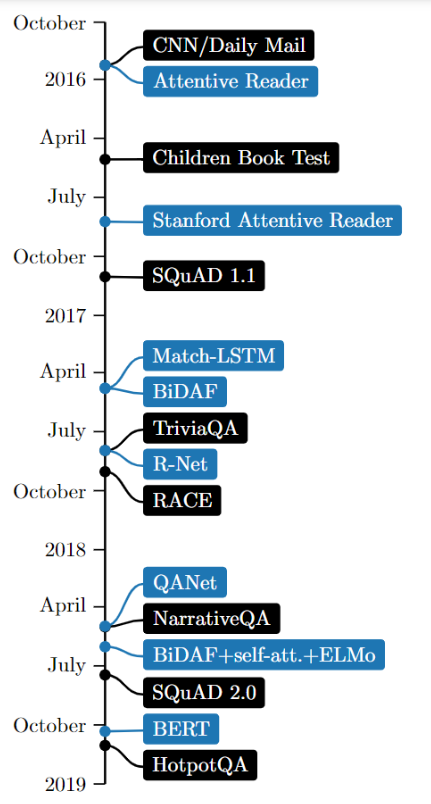
\includegraphics[height=0.8\textwidth]{figure/mrc_dev.png}
	\caption{近年深度学习机器阅读理解模型发展}
	\label{mrc_dev}
\end{figure}
\subsubsection{神经网络模型开端}
2015年,Google DeepMind的Hermann等人发表《Teaching Machines to Read and Comprehend》\upcite{teaching},其中提出了三种神经网络模型:Deep LSTM,Attentive Reader,Impatient Reader,作为baseline。
其中各个模型的特点:
\begin{enumerate}
	\item \textbf{Deep LSTM} 将doc和query进行拼接(doc|||query 或者 query||| doc)实际上视作一个长文本,用多层的LSTM来encode,得到最后的隐藏层状态,进而进行后面的任务。
	\begin{figure}[H]
		\centering
		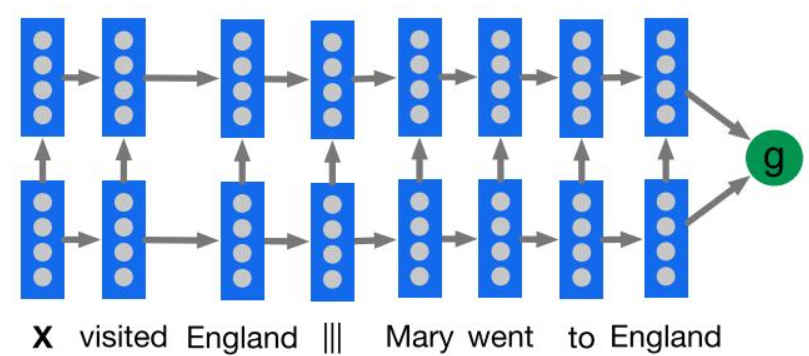
\includegraphics[width=0.5\textwidth]{figure/lstm.png}
		\caption{Deep LSTM}
		\label{model_lstm}
	\end{figure}
	\item \textbf{Attentive Reader} 在LSTM的基础上,引入attention的概念,将doc和query分开表示。每个部分用双向的LSTM来encode。Query用两个方向上的last hidden state进行表示,doc中每个token用两个方向的hidden state表示,而doc用每个token的加权来表示,其权重即为attention。
	\begin{figure}[H]
		\centering
		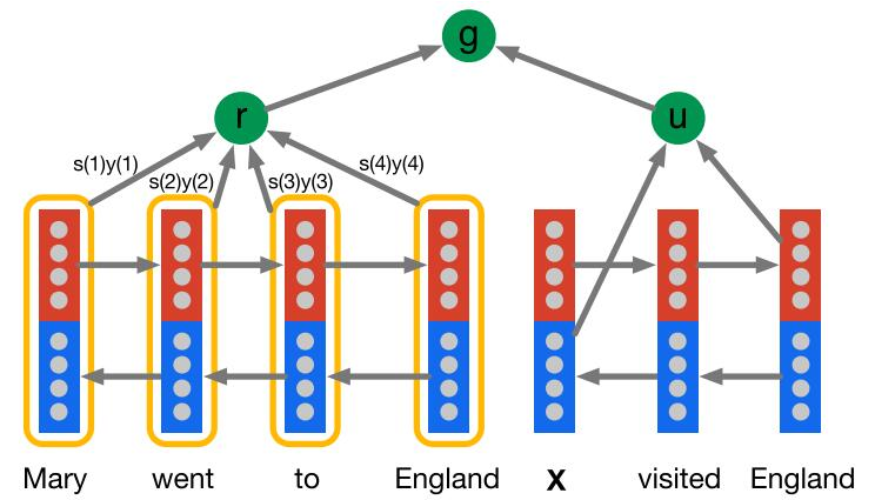
\includegraphics[width=0.5\textwidth]{figure/attentive.png}
		\caption{Attentive Reader}
		\label{model_attentive}
	\end{figure}
	\item \textbf{Impatient Reader} 相对于Attentive Reader模型,不再将整个query考虑为整体,每个query token都与document tokens有关联。
	\begin{figure}[H]
		\centering
		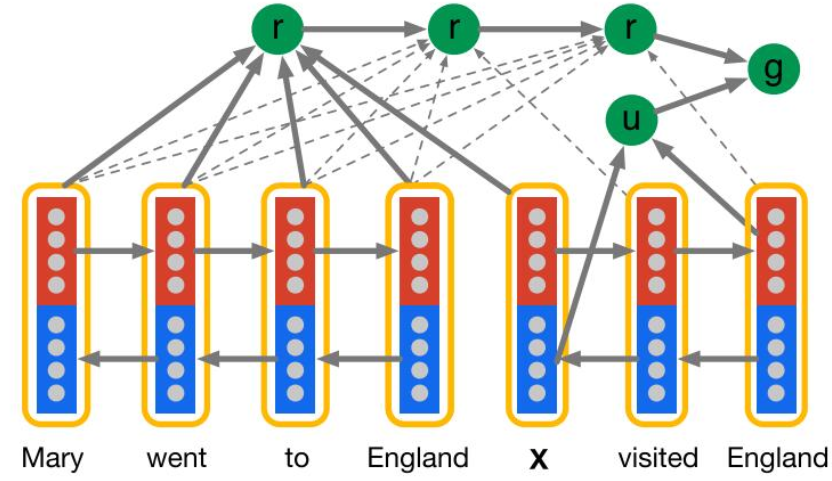
\includegraphics[width=0.5\textwidth]{figure/impatient.png}
		\caption{Impatient Reader}
		\label{model_impatient}
	\end{figure}
\end{enumerate}

\subsubsection{BiDAF}
BiDAF(Bi-directional Attention Flow)\upcite{bidaf}在Attentive Reader上的主要改进如下:
\begin{enumerate}
	\item 没有将context 压缩到一个 fixed-size 向量,而是在每个 time step 上计算 attention。 并且允许每层的向量表示能够传递到后续层,减少了信息损失。
	\item 采用无记忆注意力机制,即在当前time step 的注意力并不依赖于之前的注意力的值。
	\item 使用了双向注意力机制。计算了 query-to-context(Q2C) 和 context-to-query(C2Q)两个方向的 attention 信息,认为 C2Q 和 Q2C 实际上能够相互补充。
\end{enumerate}
\begin{figure}[H]
	\centering
	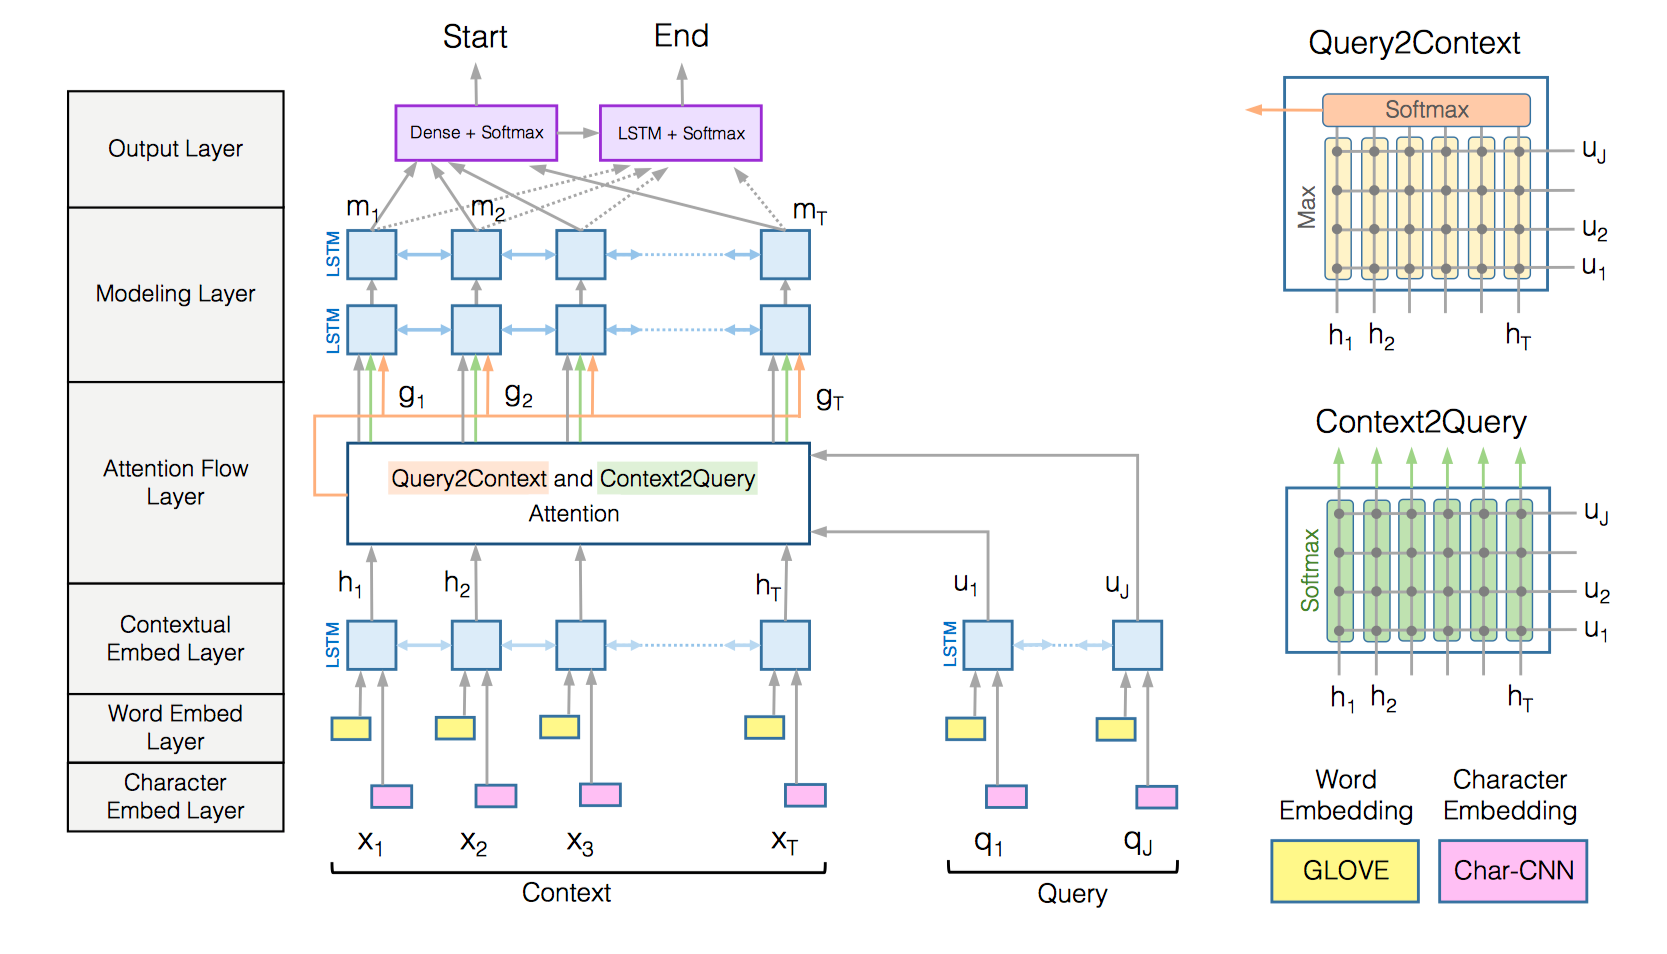
\includegraphics[width=0.6\textwidth]{figure/bidaf.png}
	\caption{BiDAF}
	\label{bidaf}
\end{figure}

\subsubsection{R-net}
R-net\upcite{rnet}是由微软提出的,在前面模型上的主要改进如下:
\begin{enumerate}
	\item encoder 中加入Gated Match-LSTM模块,可以理解为通过gate过滤掉输入中跟问题和答案不相关的部分。
	\item 增加了第三层:文章的自匹配注意力层,使得文章内部的词与词之间相互融合, 通过自身上下文信息辅助筛选有价值的词,在模型效果提升中起到了很大的作用。
\end{enumerate}
但是R-net只使用了单向的attention,仍然有改进的空间。

\begin{figure}[H]
	\centering
	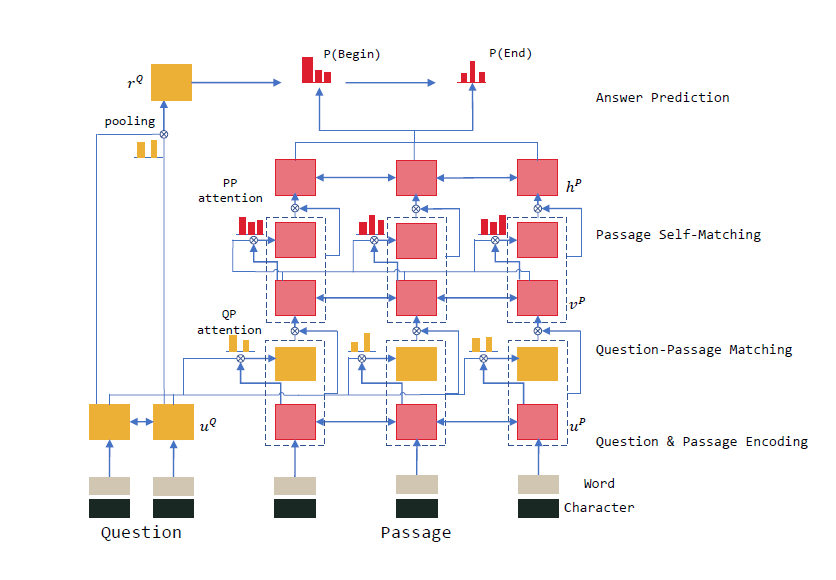
\includegraphics[width=0.6\textwidth]{figure/rnet.png}
	\caption{R-net}
	\label{rnet}
\end{figure}
\subsubsection{QA-net}
QA-net\upcite{qanet}是谷歌提出的一个模型。之前阅读理解的端到端模型主要都是基于RNN的,所以在训练和预测上运行较慢,所需资源较多。而QANet不需要RNN构成,显著地提高了训练速度和预测速度。在前面模型上的主要改进:在Embedding Encoder Layer和Model Encoder Layer中使用encoder block,单个encoder block结构自底向上依次包含位置编码(position encoding),卷积(conv)层,self attention层和前馈网络(fnn)层。卷积能够捕获上下文局部结构,而self-attention则可以捕捉文本之间全局的相互作用。因此QA-net的特点是训练快,但内存需求较大。

\begin{figure}[H]
	\centering
	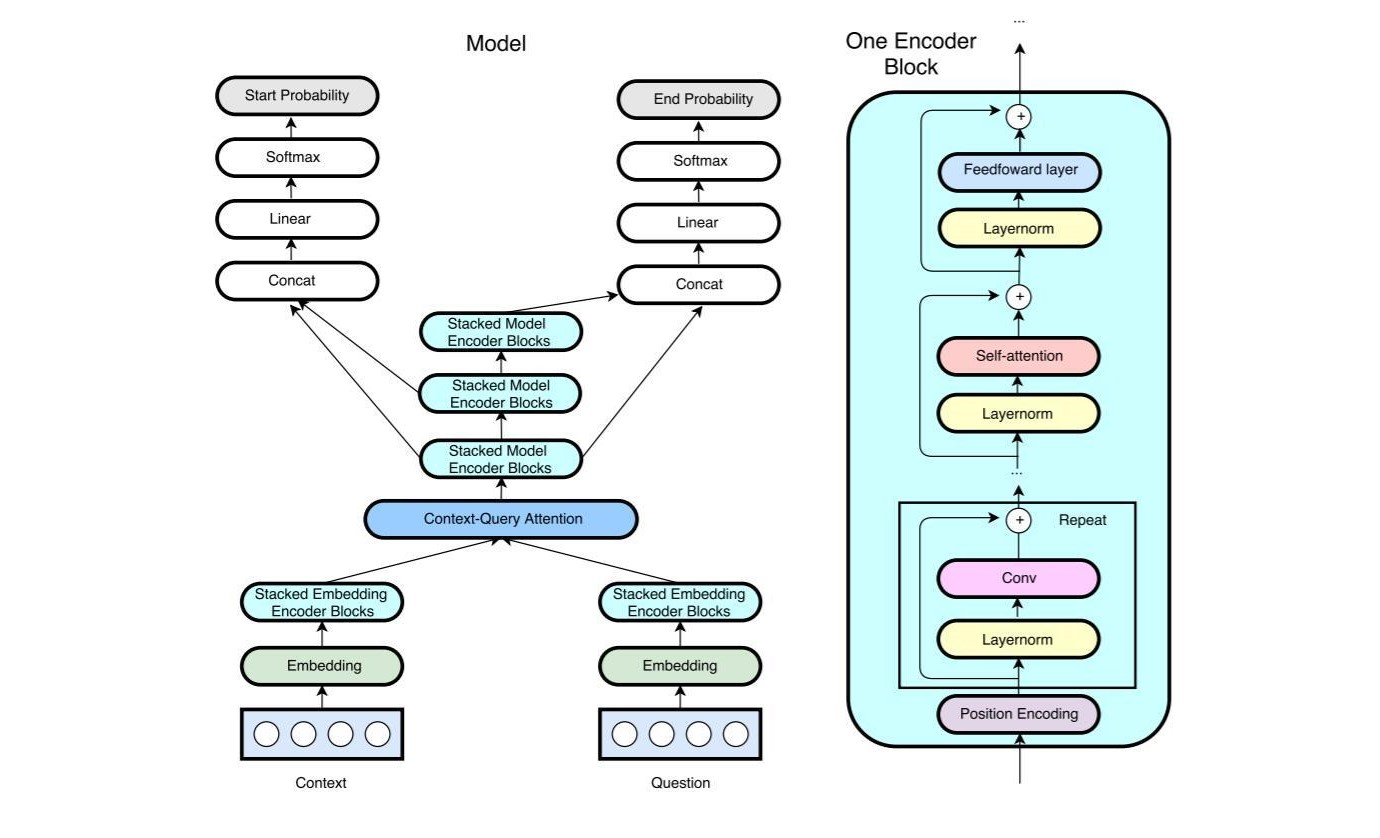
\includegraphics[width=0.6\textwidth]{figure/qanet.jpeg}
	\caption{QA-net}
	\label{qanet}
\end{figure}

\section{模型介绍}
\subsection{BERT}
\subsubsection{Bert模型介绍}
BERT模型\upcite{bert}为谷歌提出的一个预训练的模型,具备广泛的通用性,刷新了很多NLP任务的最好性能。预训练,即用大语料训练出语言模型,将其迁移到特定任务,从而进行特征维度的迁移,句子级别信息的迁移。

BERT模型采用Transformer Encoder作为语言模型,完全采用注意力机制来进行input-output间的计算,完全抛弃了RNN/CNN等结构。
BERT模型主要是在OpenAI的GPT上发展而来的,主要区别在于采用了Transformer Encoder,也就是在每个时刻的Attention计算都能够得到全部时刻的输入;而GPT采用了Transformer Decoder,每个时刻的Attention计算只能依赖于该时刻前的所有时刻的输入,因为GPT是采用了单向语言模型。而BERT使用了双向语言模型,能够同时获得上下文信息。这里,需要说一下,在最近的GPT2.0中,仍然采用的是单向语言模型,其效果依然很好,因此语言模型的单向和双向哪个更好,仍然有待讨论。

\begin{figure}[H]
	\centering
	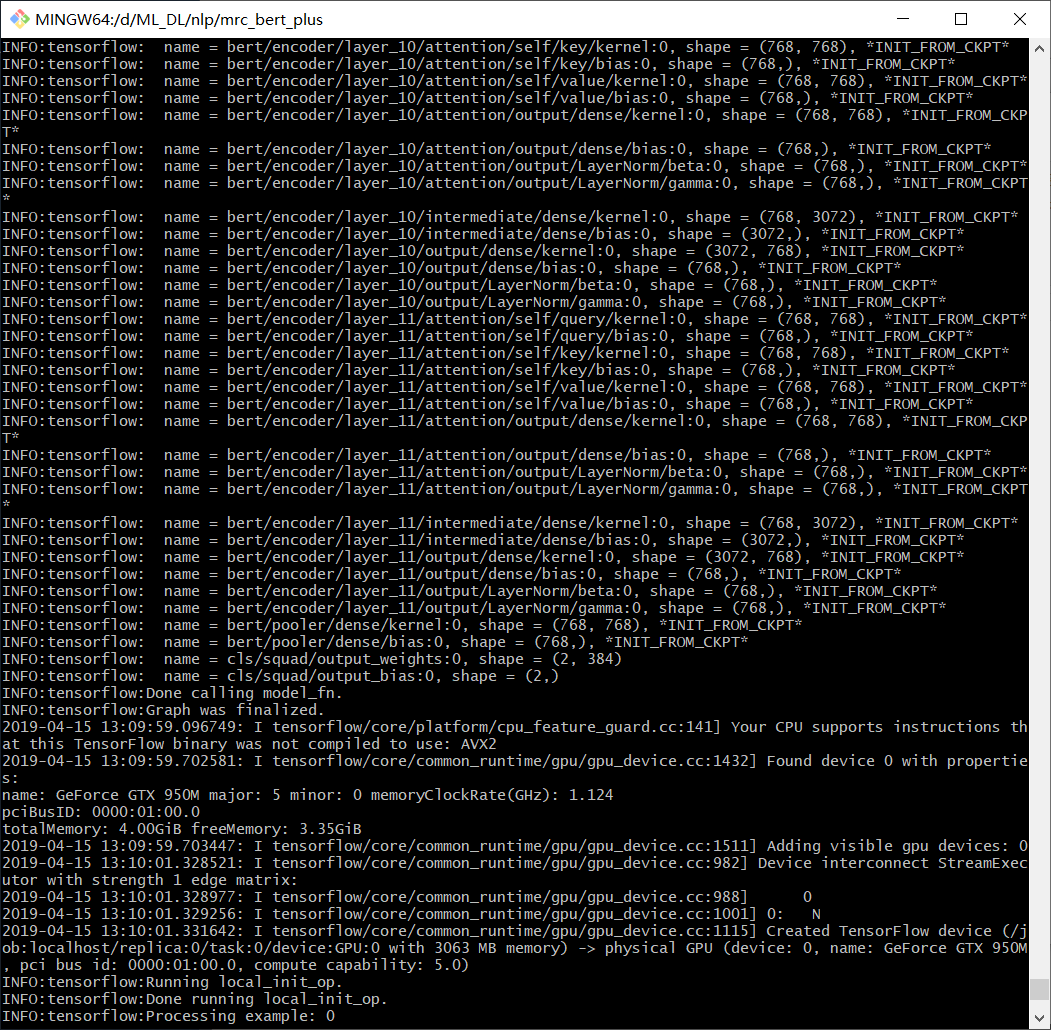
\includegraphics[width=0.6\textwidth]{figure/bert.jpg}
	\caption{BERT与其他预训练模型的对比}
	\label{bert_compare}
\end{figure}
\subsubsection{BERT模型的预训练任务}
为了能够有利于token-level任务(如:序列标注)和sentence-level任务(如:情感分析,问答系统等),BERT模型采用了两个预训练任务:
\begin{enumerate}[fullwidth,itemindent=2em,label=(\arabic*)]
	\item \textbf{Masked Language Model\ }  随机去掉句子中的部分token,然后模型来预测被去掉的token。使用该模型,可以利用双向的信息,即同时利用好前面词和后面词的概率。
	\item \textbf{Next Sentence Prediction\ }  很多需要解决的NLP tasks依赖于句子间的关系,而这个关系语言模型是获取不到的,因此将下一句话预测作为了第二个预训练任务。该任务的训练语料是两句话,来预测第二句话是否是第一句话的下一句话。
\end{enumerate}
\begin{figure}[H]
	\centering
	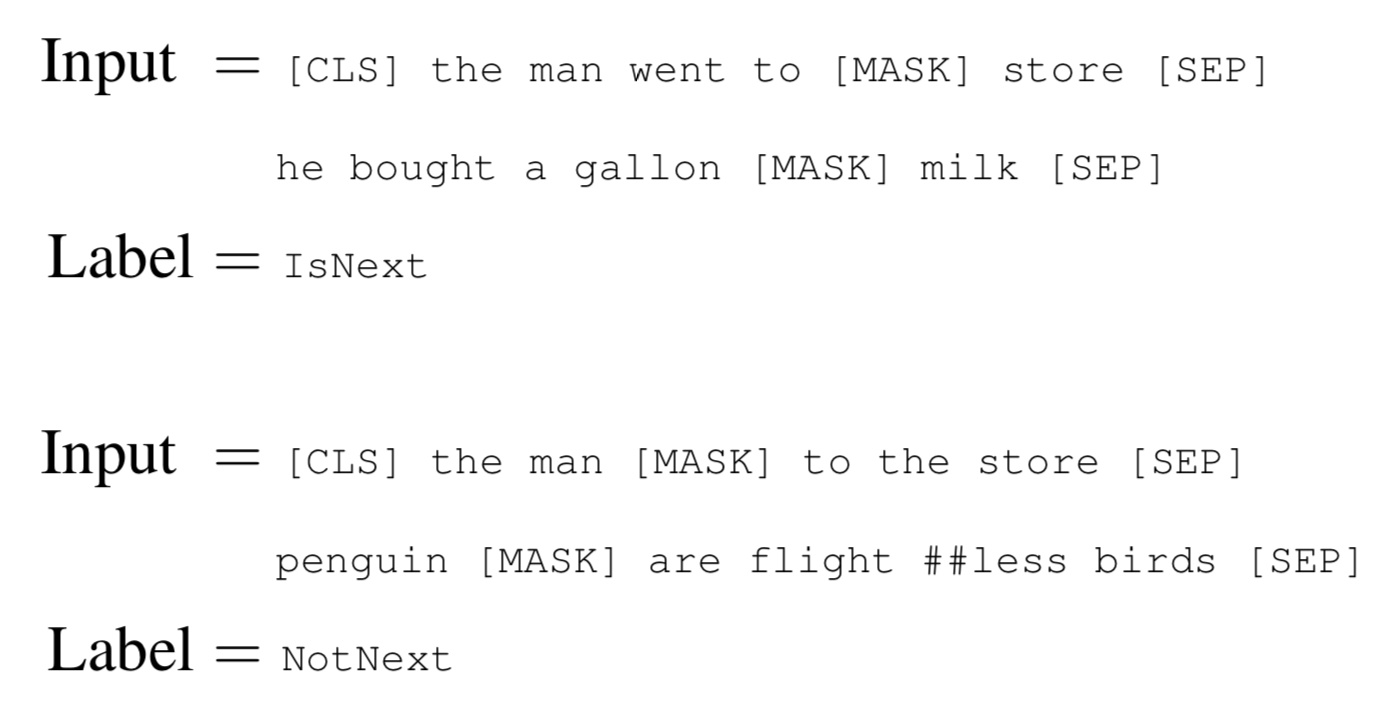
\includegraphics[width=0.4\textwidth]{figure/next.png}
	\caption{Next Sentence Prediction样例}
	\label{next}
\end{figure}
在训练过程中,将这两个任务的loss相加,作为总的loss进行优化。

\subsubsection{BERT模型fine tuning}
如图\ref{fine_tuning},原论文给出了几类任务的fine tuning方法,主要包括:句子对分类、单句分类、QA问答、序列标注等任务。在本次阅读理解任务中,主要采用\ref{fine_tuning}中(c)方法,将问题和文章结合作为模型输入,输出结果为文章中每个单词作为答案边界的概率。
\begin{figure}[H]
	\centering
	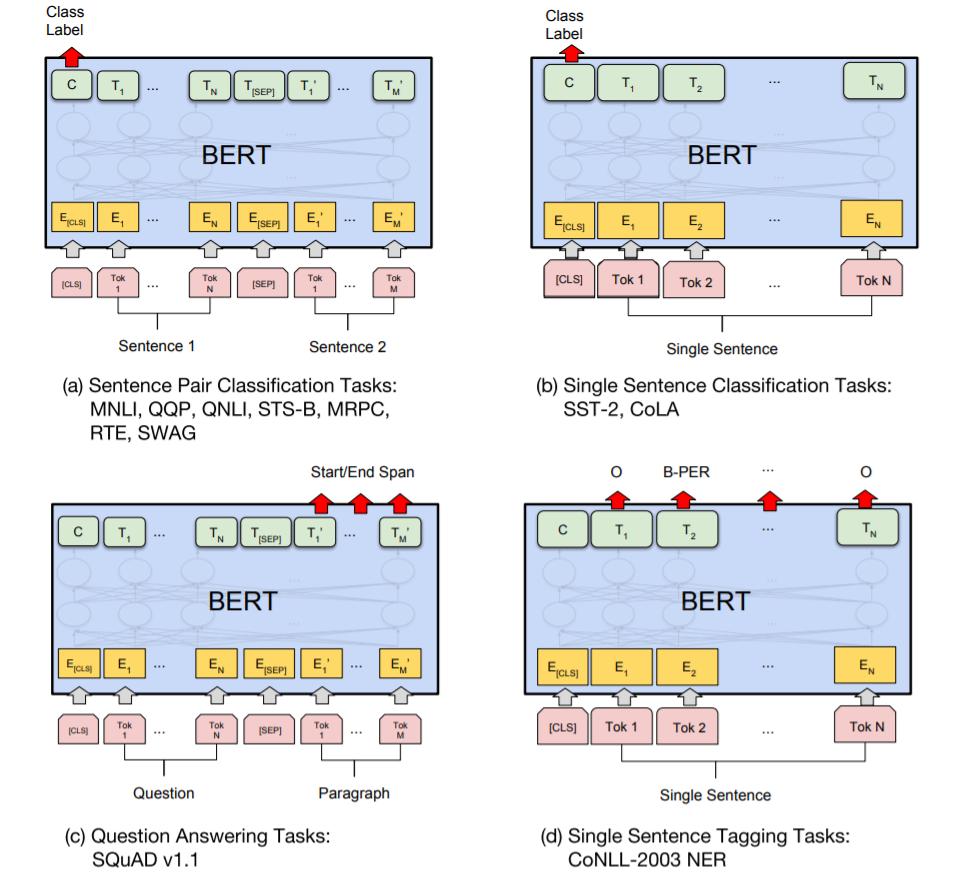
\includegraphics[width=0.5\textwidth]{figure/Bert_fine_tuning.png}
	\caption{Bert fine tuning}
	\label{fine_tuning}
\end{figure}


\subsection{BERT+R-net}
实验过程中,R-net部分和论文中的原始实现没有太大差别。只是将embedding层用了BERT表示,鉴于BERT的训练特性,因此在embedding时,将问题和文章一起编码,问题放在前面,文章放在后面,形式如下:
$$
[CLS]Query[SEP]Context[SEP]
$$
由于BERT训练时采用了Predict Next Sentence的方式,因此,将问题放在文章前面,训练时能够得到更加丰富的信息,有利于之后的答案提取。

而在R-net中的Context和Query的attention部分,分别需要Query和Context的向量表示,此时选择将BERT的embedding结果复制两份,然后使用Query和Context的mask信息,分别获得Query和Context的向量表示,然后进行attention操作。

\section{实验结果及分析}
\subsection{实验说明}
实验配置如图\ref{env}
\begin{table}[H]
	\centering
	\caption{BERT运行环境配置}
	\setlength{\tabcolsep}{1mm}{
		\begin{tabular}{ccc}
			\toprule  %添加表格头部粗线
			 & 环境 & 配置   \\
			\midrule  %添加表格中横线
			笔记本 & tensorflow-gpu=1.10 & Win10 950M (4G显存) \\
			\midrule  %添加表格中横线
			服务器 & tensorflow-gpu=1.12 & K80 (12G显存) \\
			\bottomrule %添加表格底部粗线
	\end{tabular}}
	\label{env}
\end{table}

\subsection{数据集说明}
本次任务使用的是cmrc2017\upcite{cmrc}的数据集,数据集答案主要构成是(形容词+)名词。但是给定数据集已经进行了分词,并且答案是分词中的某个词语,因此鉴于分词器的性能,答案形式不唯一,如图\ref{dataset}所示,而这将对后续的模型效果产生一定的影响。
\begin{figure}[H]
	\centering
	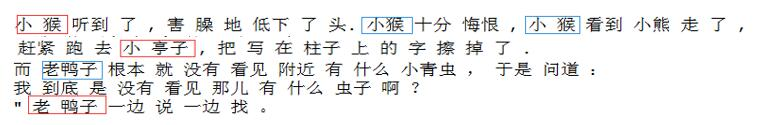
\includegraphics[width=0.8\textwidth]{figure/dataset.jpg}
	\caption{数据集举例说明}
	\label{dataset}
\end{figure}

\subsection{实验过程说明}
\subsubsection{数据增强}
实验过程中,尝试了使用回译和EDA\upcite{eda}进行数据增强,具体如下:
\begin{enumerate}
	\item \textbf{回译\ } 回译进行数据增强的主要过程是:将中文问题进行搜狗翻译\upcite{sogou}成英文,然后将获得英文问题,使用有道翻译\upcite{youdao},获得翻译之后的中文问题,最后将问题对应的原文章和翻译后所得问题作为一个样本添加到数据集中进行训练。
	\item \textbf{EDA\ } EDA数据增强,主要就是同义词替换、插入、交换和删除。
\end{enumerate}

\subsubsection{过拟合}
在实验开始,使用了BERT+R-net模型,并且在训练R-net模型的同时训练BERT模型,训练过程中loss变化如图\ref{loss},出现了严重的过拟合现象。
\begin{figure}[H]
	\centering
	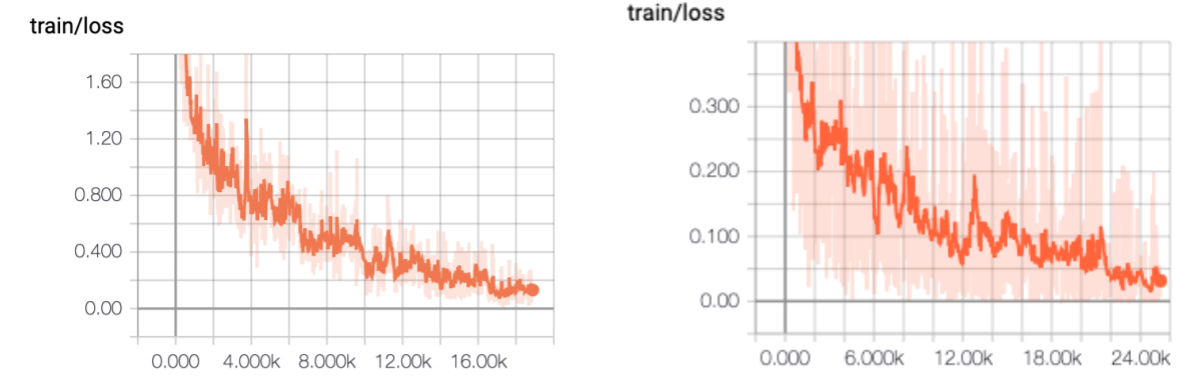
\includegraphics[width=0.8\textwidth]{figure/loss.png}
	\caption{训练过程中loss变化}
	\label{loss}
\end{figure}
主要原因在于网络模型过于复杂,参数过多,因此很容易过拟合。之后采用了以下两种变种模型:
\begin{enumerate}
	\item 如图\ref{bert_rnet1},先使用数据集在BERT上进行fine tuning;然后再使用数据集在BERT+R-net上进行训练,此时,将BERT固定,使用之前在数据集上fine tuning的参数,并且不再进行训练。
	\item 如图\ref{bert_rnet2},使用数据集训练BERT+R-net,此时,将BERT固定,使用Google给出的模型参数进行训练;训练一段时间之后,不再固定BERT,而是将BERT与R-net同时进行训练。
\end{enumerate}
\begin{figure}[H]
	\centering  %图片全局居中
	\subfigure[BERT+R-net1]{
		\label{bert_rnet1}
		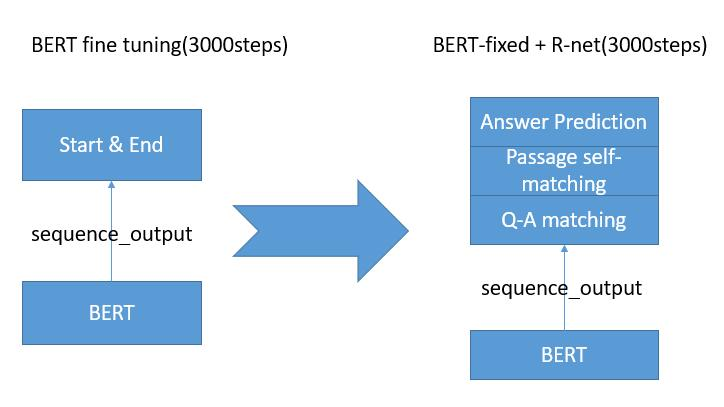
\includegraphics[width=0.4\textwidth]{figure/bert_rnet1.jpg}}
	\subfigure[BERT+R-net2]{
		\label{bert_rnet2}
		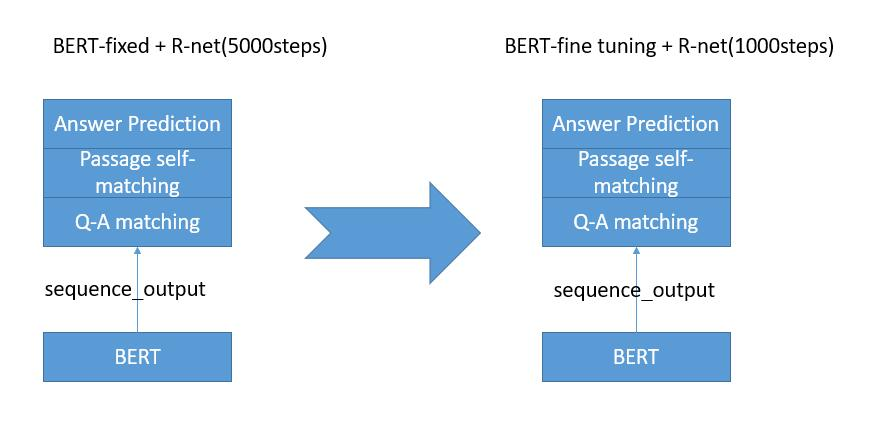
\includegraphics[width=0.4\textwidth]{figure/bert_rnet2.jpg}}
	\caption{BERT+R-net模型变种}
	\label{bert_rnet}
\end{figure}

\subsubsection{后处理}
通过分析数据集获得答案长度分布,如图\ref{length}所示。可以发现长度为2的答案最大,并且最长答案长度为5。因为,R-net输出的是文章中各个位置作为答案起点和终点的概率,因此,最终答案是随机组合获得的,所以可能出现top1答案的长度非常长,缺少限制。为了提高最终测试性能,对R-net输出的候选答案进行后处理,选择长度小于5的最优答案。
\begin{figure}[H]
	\centering
	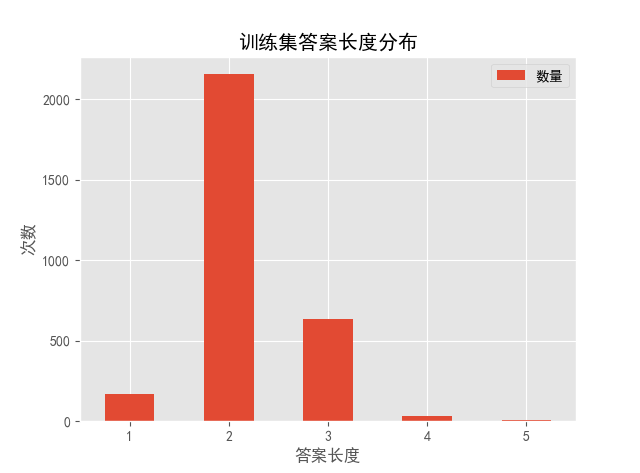
\includegraphics[width=0.6\textwidth]{figure/length.png}
	\caption{答案长度分布}
	\label{length}
\end{figure}

\subsection{实验结果及分析}
最终实验结果如图\ref{result}所示。
\begin{table}[H]
	\centering
	\caption{在测试集上结果}
	\begin{tabular}{cccc}
		\toprule  %添加表格头部粗线
		模型 & 召回率(\%)  & 准确率(\%) & F1值(\%)   \\
		\midrule  %添加表格中横线
		BERT baseline  & 86.809 & 88.479 & 86.941 \\
		+DA            & 86.151 & 86.841 & 84.166 \\
		+Context2Query & 87.365 & 88.237 & \textbf{87.752} \\
		+Answer Limit  & 87.315 & 88.546 & \textbf{87.382} \\
		+R-net1        & 84.762 & 86.233 & 85.488 \\
		+R-net2        & 86.908 & 88.401 & 86.892 \\
		\midrule  %添加表格中横线
		total          & 88.532 & 90.776 & \textbf{89.067} \\
		\bottomrule %添加表格底部粗线
	\end{tabular}
	\label{result}
\end{table}
对实验结果分析如下:
\begin{enumerate}
	\item \textbf{DA} 数据增强,包括回译和EDA两种手段。其中EDA的例子如图\ref{eda}所示,可以发现结构比较混乱,因为效果较差,因此最终并没有采用这种方法。
	\begin{figure}[H]
		\centering
		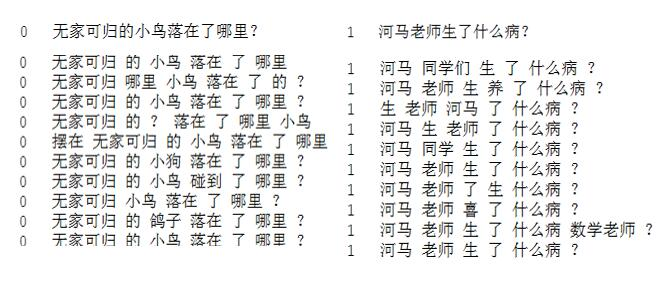
\includegraphics[width=0.65\textwidth]{figure/eda.jpg}
		\caption{EDA举例}
		\label{eda}
	\end{figure}
	实验结果中的数据增强是回译的测试结果。回译的测试效果在baseline的基础上下降了,主要在于翻译的效果受限。部分回译结果如表\ref{eda_result}。可以发现绝大多数的回译结果,都是引入了结构变化,进行语句主干成分的调整。但是,在人名和事件名回译中引入了较大的噪声,会导致之后的答案查找出现较大误差。
	\begin{table}[H]
		\centering
		\caption{回译举例}
		\begin{tabular}{cc}
		\toprule  %添加表格头部粗线
		原问题 & 回译结果  \\
		\midrule  %添加表格中横线
		国与国之间会把谁作为人质?& 谁将在国与国之间成为人质?  \\
		羊和狼的盟约以什么作为保证?& 羊和狼结盟的保证是什么? \\
		小兔和谁是好朋友?& 谁是兔子的好朋友? \\
		 我最好的朋友是谁? & 谁是我最好的朋友?  \\
		美丽的湖泊是什么构成的?   & 什么构成了一个美丽的湖?  \\
		\midrule  %添加表格中横线
		 老鼠发现小朋友小毛在干什么? & 当老鼠发现小男孩的头发时,它在做什么? \\
		 伍奢的第二个儿子是谁?  & 吴舍是谁的二儿子?  \\
		 吕后指定谁为相国?  &  吕侯任命谁为宰相? \\
		 第三次中东战争前夕,洛茨来到了哪里?  & 在六日战争前夕,罗兹到哪里去了?  \\
		\midrule  %添加表格中横线
		 树林中有什么?  & 那里是什么?在树林里。  \\
		 山洞里住着一只什么?    & 那里住着什么?里面是一个洞穴  \\
		\bottomrule %添加表格底部粗线
		\end{tabular}
		\label{eda_result}
	\end{table}
	同时,回译的方式有待商榷,仅仅对问题进行回译,可能意义不是很大,需要进行更细致的甄别和思考。
	\item \textbf{Context2Query} 在BERT baseline上引入了文章对问题的attention,主要是对于文章中的每个词求对问题中每个词的attention,然后通过计算得到的信息获得文章的向量。在这个实验中,测试结果在BERT baseline上获得了微小的提升。主要原因在于BERT本身使用了大量的attention机制,而再加入attention机制后,起到的作用不是很大。
	\item \textbf{Answer Limit} 在对标准答案进行了分析之后,选择对于top N的答案进行额外分析,选择在最大答案长度限制内的最优答案最为最终答案。由于BERT的最终结果进行了概率组合,因此部分答案可能不是很规范,会很长,因此进行了答案长度限制后,效果得到的提升。
	\item \textbf{R-net1} 在这个模型中,同时训练了BERT+R-net,导致网络模型很复杂,因此出现了严重的过拟合,最终测试效果不太好,比BERT baseline差。
	\item \textbf{R-net2} 为了解决模型复杂过拟合的问题,对BERT+R-net进行的修改,不进行同时训练。此处选择,先使用训练集对BERT进行fine tuning。然后在BERT+R-net模型中,固定BERT,并且使用fine tuning时的模型参数进行初始化,以减少模型训练量。最终测试效果和BERT baseline相当。
	\item \textbf{total} 将最终所有的增益模型进行相加测试,测试结果得到提升。
\end{enumerate}

\subsection{可视化应用}
在课程中,为了更好的展示实现效果,进行了可视化应用开发。应用主要包括问题获取、问题理解、问题回答三部分。其中,问题获取部分,支持用户进行文章选择,并且使用了讯飞的语音识别API,进行用户的语音提问到文本的转化;问题理解部分,调用BERT+R-net模型,进行阅读理解和答案预测;问题回答部分,将模型的答案在原文中标出,同时调用了讯飞的语音合成API进行文本到语音的转换,最终反馈给用户。
\begin{figure}[H]
	\centering
	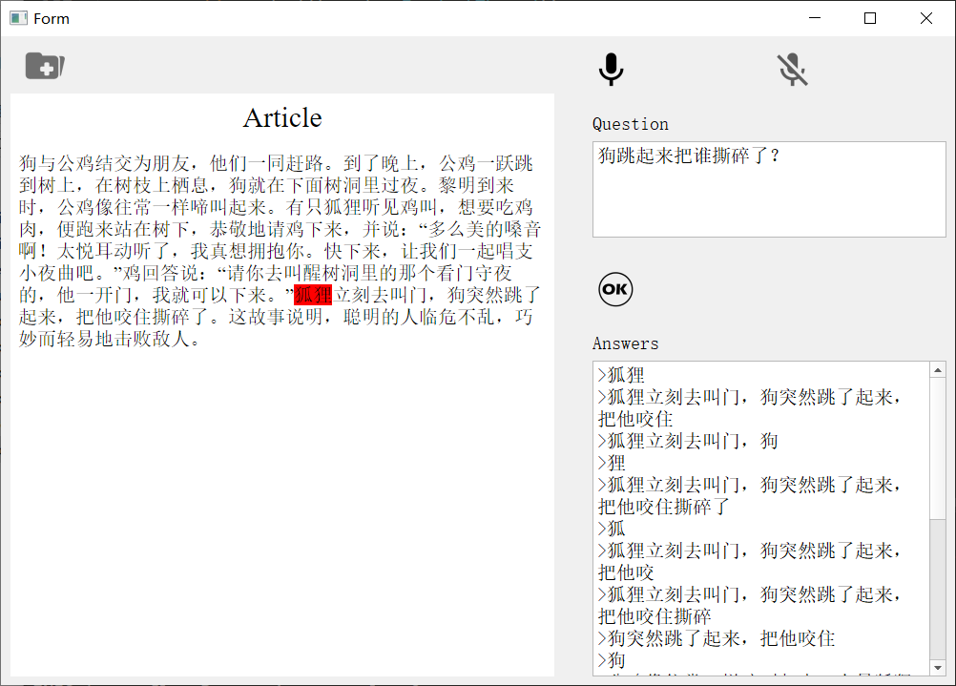
\includegraphics[width=0.5\textwidth]{figure/visual.png}
	\caption{可视化应用截图}
	\label{visual}
\end{figure}

\section{结束语}
\subsection{总结}
在本次课程中,主要使用了BERT模型完成机器阅读理解任务,在整个过程中,循序渐进,收获颇丰。课程开始,对于机器阅读理解任务知之甚少,也不了解BERT模型,花了较长的时间进行技术调研,然后阅读BERT代码和相关论文,逐渐增加了对BERT的理解,同时也能够使用BERT搭建阅读理解任务的baseline,并且效果比较理想。课程的中间阶段,主要进行了模型的改进。由于在以前的学习中基本都是使用的Keras进行的神经网络模型搭建,而课程中使用Tensorflow不是很熟练,因此遇到了很多问题,花费了较长时间进行相关资料的查询和学习。幸运的是,最终完成了在BERT基础上搭建其他神经网络模型的任务,实现了BERT+R-net的模型,并且之后在老师和学长的建议下,进行了相关改进,后续过程中,进一步增加了对于模型的理解,也学习到了很多新知识和技能。虽然最终改进效果没有达到我的预期,但是在这个过程中,实践的经验是是宝贵的,学习到的知识是无价的。

总的来说,通过这次课程,坚定了我在NLP道路上前进的信念,明确了前进的方向,对我之后的学习和研究有着指导性的意义。
最后,感谢老师们和助教在课程中的指导和建议,同时也感谢我的队友的支持、帮助和信任!

\subsection{下一步}
\begin{enumerate}[fullwidth,itemindent=2em,label=(\arabic*)]
	\item \textbf{BERT + R-net\ } 在解决BERT+R-net的过拟合问题时,可以选择不同时训练BERT和R-net。课程中,使用了cmrc数据集预训练BERT模型,之后使用BERT模型提取embedding,输入到R-net中进行训练。不同时训练BERT和R-net,可以降低网络模型的复杂度,有效避免过拟合。在以后的学习中可以采取前文中提到的第二种训练方式,即使用google提供的BERT预训练模型,在训练BERT+R-net时不改变BERT模型的参数,训练一段时间后,再开启BERT模型的参数训练,这种训练方式理论上和前一种方式差不多。
	\item \textbf{BERT + +\ } 在课程中,主要使用了BERT+R-net模型。而实际上,目前在SQUAD\upcite{squad2.0}上,高居榜首的是BERT+AoA,在某种程度上,效果超过了人类。在以后的学习中,可以研究Attention Over Attention\upcite{cui2016attention}模型,进行相关的实验。
	\item \textbf{ERNIE模型\ } BERT是基于字进行训练的,但是中文一般是以词为单位的。因此,单独使用基于词的训练,可能会失去词的语义知识。在不久以前,百度在BERT模型基础了,在中文语料上,基于词进行了训练ERINE\upcite{ernie}。ERNIE通过建模海量数据中的词、实体及实体关系,学习真实世界的语义知识。相较于 BERT 学习原始语言信号,ERNIE 直接对先验语义知识单元进行建模,增强了模型语义表示能力。训练数据方面,除百科类、资讯类中文语料外,ERNIE 还引入了论坛对话类数据,利用 DLM(Dialogue Language Model)建模 Query-Response 对话结构,将对话 Pair 对作为输入,引入 Dialogue Embedding 标识对话的角色,利用 Dialogue Response Loss 学习对话的隐式关系,进一步提升模型的语义表示能力。ERNIE在自然语言推断,语义相似度,命名实体识别,情感分析,问答匹配 5 个公开的中文数据集合上进行了效果验证,ERNIE 模型相较 BERT 取得了更好的效果。在以后的学习中,可以尝试使用ERNIE模型。
\end{enumerate}

\renewcommand{\refname}{参考文献}
%按引用的先后顺序排序
\bibliographystyle{unsrt}
\bibliography{cites}%%我们的例子应该是\bibliography{cited}

\end{document}
